%--------------------------------------------------------------------%
%
% Berkas utama templat LaTeX.
%
% author Petra Barus, Peb Ruswono Aryan
%
%--------------------------------------------------------------------%
%
% Berkas ini berisi struktur utama dokumen LaTeX yang akan dibuat.
%
%--------------------------------------------------------------------%

\documentclass[12pt, onecolumn, oneside, final]{book}

\usepackage{config/if-itb-thesis}

\bibliography{references}

\begin{document}
    \frontmatter
    %Basic configuration
    \title{Kriptografi Paralel}
    \date{Oktober 2017}
    \author{
        Muhammad Reza Ramadhan \\
        NIM 13514107
    }

    \input{chapters/cover}
    \clearpage
\pagestyle{empty}

\begin{center}
\smallskip

    \Large \bfseries \MakeUppercase{\thetitle}
    \vfill

    \Large Laporan Tugas Akhir
    \vfill

    \large Oleh

    \Large \theauthor

    \large Program Studi Teknik Informatika \\
    Sekolah Teknik Elektro dan Informatika \\
    Institut Teknologi Bandung \\

    \vfill
    \normalsize \normalfont
    Telah disetujui dan disahkan sebagai Laporan Tugas Akhir di Bandung, pada tanggal 20 Juli 2016.

    \vfill
    \setlength{\tabcolsep}{12pt}
    \begin{tabular}{c@{\hskip 0.5in}c}
        Pembimbing I, & Pembimbing II \\
        & \\
        & \\
        & \\
        & \\
        Dr. Ir. Rinaldi Munir, MT. & Dr. Judhi Santoso M.Sc. \\
        NIP 196512101994021001 & NIP 196302041989031002 \\
    \end{tabular}

\end{center}
\clearpage

    \input{chapters/statement}

    \pagestyle{plain}

    % \input{chapters/abstract-id}
    % \input{chapters/abstract-en}
    % \input{chapters/forewords}

    \tableofcontents
    \listoffigures
    \listoftables

    %----------------------------------------------------------------%
    % Konfigurasi Bab
    %----------------------------------------------------------------%
    \renewcommand{\chaptername}{BAB}
    \renewcommand{\thechapter}{\Roman{chapter}}
    %----------------------------------------------------------------%

    %----------------------------------------------------------------%
    % Dafter Bab
    % Untuk menambahkan daftar bab, buat berkas bab misalnya `chapter-6` di direktori `chapters`, dan masukkan ke sini.
    %----------------------------------------------------------------%

    % Set numbering
    \mainmatter

    \chapter{Pendahuluan}


\section{Latar Belakang}

Transport Layer Security (TLS) merupakan sebuah protokol yang banyak digunakan untuk menjamin keamanan dan kerahasiaan dari sebuah pesan yang dikirim melalui jaringan. Saat ini, TLS digunakan sebagai sebuah layer security dari berbagai protokol yang saat ini umum digunakan di Internet seperti Hyper-Text Transfer Protocol (HTTP), File Transfer Protocol (FTP), ataupun Simple Mail Transfer Protocol (SMTP). Mengingat posisi protokol ini sebagai sebuah layer yang berbeda dibandingkan protokol-protokol lain yang digunakan dalam perangkat lunak, TLS juga dapat digunakan dalam protokol lain yang mungkin dibuat pada masa yang akan datang.

Secara sederhana, sebuah koneksi TLS akan didahului dengan adanya TLS handshake untuk menentukan symmetric key yang akan digunakan oleh client dan server untuk berkomunikasi setelahnya. Sayangnya, waktu yang digunakan untuk TLS handshake masih cukup signifikan. Penggunaan TLS diatas HTTP dapat mengakibatkan waktu load pada sebuah website menjadi 1,2 hingga 3 kali lebih lambat (Naylor et al, 2014). Hal ini merupakan salah satu alasan kenapa saat ini TLS belum digunakan oleh seluruh layanan yang ada di internet.

Pada sebuah TLS handshake, client akan melakukan koneksi terhadap server untuk menandakan bahwa ia ingin membuat sebuah TLS session baru yang akan digunakan untuk pengiriman data antara client dan server. Server kemudian akan membalas koneksi tersebut dengan sebuah certificate berisi public key miliknya. Client kemudian akan membuat sebuah pre-master symmetric key yang akan dienkripsi dengan public key yang diterima. Server kemudian akan mendekripsi data yang ia terima untuk mendapat pre-master symmetric key; pre-master symmetric key akan dilakukan komputasi lebih jauh untuk mendapatkan symmetric key yang akan digunakan pada komunikasi antara server dan client.

Dari beberapa langkah yang dilakukan dalam sebuah TLS handshake, komputasi dekripsi algoritma Rivest–Shamir–Adleman (RSA) merupakan salah satu bagian dapat dioptimasi dengan relatif mudah.  Terdapat beberapa cara yang telah disarankan untuk meningkatkan kinerja TLS handshake seperti melakukan batching pada dekripsi RSA di server, melakukan rebalancing sehingga komputasi pada client lebih sulit daripada server, ataupun melakukan optimisasi pada algoritma RSA sehingga komputasi dapat dilakukan dengan lebih cepat.

Saat ini telah terdapat beberapa implementasi RSA dalam algoritma pemrograman paralel baik dalam paralel dalam Central Processing Unit (CPU) maupun dalam Graphics Processing Unit (GPU). Pembuatan algoritma RSA secara multiprocessing dalam GPU bukanlah hal yang baru dan dapat menghasilkan troughput hingga 45 kali dari implementasi RSA pada CPU (Zhang et al, 2014). Namun mengingat sebagian besar server pada data center tidak memilki GPU, implementasi RSA pada GPU tidak dapat digunakan untuk meningkatkan kinerja TLS handshake.

Dewasa ini, penggunaan CPU dengan jumlah core yang tinggi pada server merupakan hal yang lumrah; seri Xeon dari Intel telah menyediakan jumlah core hingga 22. Jumlah core yang tinggi merupakan salah satu alasan mengapa penggunaan algoritma multiprocessing pada dekripsi RSA dapat meningkatkan kinerja dari sebuah TLS handshake.


\section{Rumusan Masalah}

Kinerja dari TLS handshake hingga saat ini masih merupakan salah satu hal yang menghambat implementasi TLS secara luas. Salah satu cara untuk meningkatkan kinerja dari TLS handshake adalah dengan melakukan optimasi pada algoritma dekripsi RSA. Akan tetapi, optimisasi algoritma RSA menggunakan pemrograman paralel pada CPU bukan merupakan topik yang banyak dibahas pada penelitian-penelitian saat ini. Maka dari itu, tugas akhir ini akan berfokus pada pengembangan algoritma RSA dalam pemrograman paralel dan implementasinya pada TLS handshake. Dalam pengembangannya, terdapat berapa masalah yang akan menjadi perhatian utama dalam tugas akhir ini, yaitu:

\begin{enumerate}
  \item Algoritma paralel seperti apa yang akan diimplementasikan?
  \item Bagaimana cara mengintegrasikan algoritma paralel tersebut ke dalam TLS handshake?
  \item Apakah penggunaan algoritma paralel dapat meningkatkan kinerja dari TLS handshake?
\end{enumerate}

\section{Tujuan}

Tujuan dari tugas akhir ini adalah menemukan sebuah algoritma paralel RSA yang dapat diimplementasikan pada TLS handshake. Dengan adanya algoritma paralel tersebut, diharapkan bahwa kinerja dari TLS handshake akan meningkat dan penggunaan TLS pada internet akan semakin banyak digunakan.

\section{Batasan Masalah}

Tugas akhir ini hanya membahas mengenai optimisasi algoritma RSA pada implementasi TLS handshake. Dengan demikian, tugas akhir tidak memperhatikan hal-hal berikut:

\begin{enumerate}
  \item Protokol pertukaran kunci TLS handshake.
  \item Proses pemilihan dan/atau pembuatan cipher suite, TLS session, dan simmetric key pada TLS.
  \item Proses enkripsi pre-master symmetric key pada TLS client.
  \item Kompresi data.
\end{enumerate}

\section{Metodologi}

Pengerjaan tugas akhir ini akan melalui beberapa tahap, yaitu:
\begin{enumerate}
  \item Analisis Masalah

  Tugas akhir akan dimulai dengan dilakukannya analisis mengenai masalah terhadap implementasi TLS handshake yang ada pada saat ini. Pada tahap ini akan dipelajari juga mengenai solusi-solusi untuk meningkatkan kinerja dari TLS handshake yang sudah tersedia pada saat ini. Dari solusi yang sudah ada tersebut, penulis akan mencari penyebab solusi itu belum diimplementasikan pada TLS handshake dan mencari solusi baru yang mungkin untuk diimplementasikan.

  \item Perancangan Solusi dan Pengujian

  Perancangan solusi dibuat sebagai kerangka dasar atas solusi dari masalah yang telah ditemukan pada langkah sebelumnya. Pada tahap ini akan dirancang arsitektur solusi beserta cara untuk menerapkannya pada TLS handshake yang sudah ada. Selain itu, akan dibuat juga rencana pengujian terhadap implementasi solusi. Rencana pengujian akan dibuat sehingga percobaan dilakukan dalam batas masalah yang ada dan dapat dilakukan sesuai metode sains.

  \item Implementasi Solusi

  Pada tahap ini, penulis akan mengimplementasikan rancangan solusi yang sudah dibuat dalam sebuah bentuk perangkat lunak yang dapat digunakan dalam dunia sehari-hari. Hasil implementasi yang dibuat tentu ditujukan untuk menyelesaikan masalah yang ada.

  \item Pengujian dan Evaluasi

  Pengujian akan dilakukan berdasarkan rancangan pengujian telah ada. Pengujian dilakukan untuk mengetahui apakah solusi yang diberikan merupakan solusi terbaik dari masalah yang ada. Hasil dari pengujian akan digunakan sebagai data evaluasi dan penarikan kesimpulan.

\end{enumerate}


\section{Sistematika Laporan}

Penulisan tugas akhir ini akan terdiri dari lima bab yaitu: BAB I Pendahuluan, BAB II Studi Literatur, BAB III Analisis Solusi, BAB IV Rancangan, Implementasi dan Pengujian, BAB V Penutup.

Bab satu memaparkan mengenai latar belakang pembuatan tugas akhir ini, masalah utama yang dibahas, tujuan pembuatan tugas akhir, serta metodologi yang akan dilakukan selama pembuatan tugas akhir. Bab ini dibuat sebagai pendahuluan dan akan mencakup ringkasan dari sebagian besar hal yang dibahas pada tugas akhir.

Bab dua akan membahas mengenai teori dasar yang sudah ada mengenai protokol TLS, algoritma RSA, serta pengembangan dari algoritma RSA melalui pemrograman paralel yang sudah ada. Teori yang diambil akan bersumber dari literatur terpercaya serta dokumentasi resmi dari protokol TLS.

Bab tiga menggambarkan solusi yang digunakan untuk menyelesaikan masalah yang ada, kenapa digunakan solusi tersebut, serta hipotesa peningkatan kinerja dari TLS handshake setelah solusi yang dibuat diimplementasikan.

Bab empat memperlihatkan rancangan implementasi dari solusi, proses implementasi solusi tersebut, serta hasil pengujian dari implementasi tersebut pada kinerja TLS handshake.

Bab lima mendeskripsikan hasil kesimpulan dari solusi yang dibuat untuk menyelesaikan masalah serta saran yang dapat dilakukan untuk pengembangan dan perbaikan agar implementasi ini dapat menghasilkan hasil yang lebih baik.

    \chapter{Studi Literatur}

Bab Studi Literatur digunakan untuk mendeskripsikan kajian literatur yang terkait dengan persoalan tugas akhir. Tujuan studi literatur adalah:

\begin{enumerate}
    \item menunjukkan kepada pembaca adanya gap seperti pada rumusan masalah yang memang belum terselesaikan,
    \item memberikan pemahaman yang secukupnya kepada pembaca tentang teori atau pekerjaan terkait yang terkait langsung dengan penyelesaian persoalan, serta
    \item menyampaikan informasi apa saja yang sudah ditulis/dilaporkan oleh pihak lain (peneliti/Tugas Akhir/Tesis) tentang hasil penelitian/pekerjaan mereka yang sama atau mirip kaitannya dengan persoalan tugas akhir.
\end{enumerate}

\section{Kriptografi}
  Kriptografi adalah sebuah ilmu yang mempelajari cara pengiriman pesan sehingga tidak memungkinkan bagi pihak ketiga untuk membaca ataupun memanipulasi isi pesan tersebut. Kriptografi sudah digunakan sejak jaman kerajaan Romawi Kuno dengan digunakannya Caesar Cipher oleh Julius Caesar untuk berkomunikasi dengan Jendral Perangnya. Kriptografi modern berfokus pada teori matematis dan kesulitan pihak ketiga dalam membaca atau memanipulasi pesan secara komputasional.

  Pada berbagai literatur kriptografi sering dikenal beberapa istilah seperti:
  \begin{itemize}
    \item sender, yaitu pihak pengirim pesan
    \item receiver, yaitu pihak penerima pesan
    \item eavesdropper, yaitu pihak ketiga yang berusaha membaca atau memodifikasi pesan yang dikirim
    \item plaintext, yaitu pesan yang dikirim. Plaintext tidak harus merupakan sebuah teks namun dapat berupa audio, gambar, ataupun file binary.
    \item ciphertext, yaitu pesan yang telah diubah oleh algoritma tertentu
    \item enkripsi, yaitu proses pengubahan plaintext menjadi ciphertext
    \item dekripsi, yaitu proses pengubahan ciphertext menjadi plaintext
    \item key, yaitu nilai yang digunakan dalam enkripsi ataupun dekripsi
  \end{itemize}

  Pada umumnya, proses yang terjadi dalam penggunaan kriptografi pada sebuah pengiriman sebuah data adalah:
  \begin{figure}[h]
    \centering
    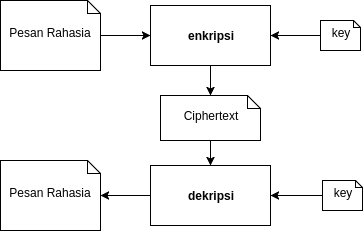
\includegraphics[width=0.6\textwidth]{resources/ch-2/crypto-system.jpg}
    \caption{Sistem Pengiriman data menggunakan kriptografi}
  \end{figure}

  Terdapat dua macam tipe kriptografi yang saat ini umum digunakan. Kriptografi kunci simetri adalah sebuah sistem kriptografi dimana proses enkripsi dan dekripsi menggunakan kunci yang sama. Kriptografi kunci publik merupakan sebuah sistem kriptografi dimana proses enkripsi dan dekripsi menggunakan dua kunci yang berbeda.

  Masalah utama yang dihadapi pada sistem kriptografi kunci simetri adalah bagaimana dua pihak dapat menentukan sebuah kunci yang akan digunakan tanpa sepengetahuan pihak ketiga. Pada algoritma kriptografi modern, terdapat beberapa metode untuk mengirimkan kunci simetri pada pihak lain, diantaranya adalah mendekripsi key tersebut dengan algoritma kriptografi kunci publik atau dengan menggunakan algoritma key exchange.

  \subsection{Kriptografi Kunci Publik}

    Kriptografi kunci publik adalah sebuah sistem kriptografi dimana proses enkripsi dan dekripsi dilakukan dengan kunci yang berbeda. Umumnya terdapat dua macam kunci yang terdapat pada sistem ini, yaitu public key yang dapat dipublikasikan kepada siapapun dan private key yang hanya dimiliki oleh pemilik kunci tersebut. Public key digunakan untuk mengenkripsi data, sementara private key digunakan oleh pemilik kunci untuk mendekripsi data tersebut.

    Salah satu kebutuhan utama yang terdapat pada kriptografi kunci publik adalah sebuah algoritma yang mudah untuk diproses dalam satu arah, namun sulit untuk dilakukan sebaliknya. Algoritma yang banyak digunakan umumnya berdasar pada masalah matematis seperti faktorisasi bilangan bulat, logaritma diskrit, atau hubungan kurva eliptik. Sebagai contoh, jika kita memiliki dua bilangan bulat maka dapat dengan mudah mengkalikan dua bilangan tesebut dan mendapat satu bilangan bulat baru; namun kita tidak bisa dengan mudah menentukan dua bilangan bulat yang merupakan faktor dari sebuah bilangan bulat.

    Namun, saat ini komputasi kriptografi kunci publik masih memerlukan proses komputasi yang lebih tinggi dibandingkan dengan kriptografi kunci simetris. Maka dari itu, kriptografi kunci publik biasanya hanya dilakukan untuk mengenkripsikan kunci yang akan digunakan dalam kriptografi kunci simetris.

    \subsubsection{Rivest–Shamir–Adleman (RSA)}

    RSA merupakan salah satu algoritma kriptografi kunci publik yang hingga saat ini banyak digunakan. Algoritma RSA pertama kali dicetuskan oleh Ron Rivest, Adi Shamir, dan Leonard Adleman pada tahun 1978. RSA berdasar pada sifat matematis bahwa dalam sebuah pemangkatan modular dengan persamaan:
    \begin{equation}
      (m^e)^d  \equiv  m \pmod{n}
    \end{equation}

    Pencarian tiga bilangan bulat n, e, dan d dapat dilakukan dengan mudah; bahkan untuk bilangan n, e, dan d yang sangat besar. Namun, pencarian bilangan d akan susah dilakukan, bahkan jika kita mengetahui bilangan-bilangan lainnya. Selain itu mengingat operasi perpangkatan dapat ditukar, maka proses enkripsi dan dekripsi dapat dilakukan dengan metode yang sama, hanya menggunakan bilangan yang berbeda.

    Terdapat beberapa proses yang terjadi pada algoritma RSA yaitu pembuatan public dan private key, distribusi public key, enkripsi, serta dekripsi. Proses pembuatan public dan private key sendiri dilakukan dalam beberapa tahap yaitu:

    \begin{enumerate}
      \item Pilih dua bilangan prima yang besar, p dan q.
      \item Hitung dan .
      \item Pilih sebuah bilangan bulat random e dengan  dan .
      \item Hitung bilangan bulat d, dengan
    \end{enumerate}

    Dari perhitungan diatas, didapat public key (e, n) dan private key d.
    Proses enkripsi pada sebuah data D dapat dilakukan melalui beberapa langkah sebagai berikut:
    \begin{enumerate}
      \item
    \end{enumerate}

\section{Aritmetika Modular}
\blindtext
\subsection{Chinese Remainder}
\blindtext
\subsubsection{Residue Number System}
\blindtext
\subsection{Repeated Square and Multiply}
\blindtext

\section{Transport Layer Security (TLS)}
\subsection{Protokol TLS Record}
\blindtext
\subsection{Protokol TLS Handshake}
\blindtext
\subsection{Ciphersuite}
\blindtext
\section{Penelitian Terkait}
\blindtext
\subsection{SSL Proxy}
\blindtext
\subsection{Implementasi Algoritma Paralel RSA}
\blindtext
\subsubsection{Penggunaan CUDA Framework}
\blindtext
\subsubsection{Repeated Square-and-Multiply}

\section{Pemrograman Paralel}
\blindtext
\subsection{Pemrograman Paralel pada Tingkat Hardware}
\blindtext
\subsubsection{Pemgrograman Paralel Pada GPU}
\blindtext
\subsection{Pemrograman Paralel pada Tingkat Software}
\blindtext
\subsubsection{Interaksi Antar Process}
\blindtext

    \chapter{Rencana Penyelesaian Masalah}

\section{Analisis Kinerja TLS}
Penggunaan TLS pada sebuah infrastrukur internet dapat membantu penjaminan keamanan dari proses keluar masuknya data. Namun, penggunaan TLS memilki harga yang mahal secara komputasi yang dilakukan, sehingga membuat kinerjanya sendiri lambat. Pengurangan kinerja dari penggunaan TLS sendiri berdampak pada 3.4 hingga 9 kali dibandingkan dengan deployment tanpa penggunaan TLS (Coarfa et. al, 2006). Mengingat beberapa tipe website seperti personal blog, portal berita, ataupun search engine tidak benar-benar membutuhkan keamanan informasi, tidak sedikit dari situs tersebut yang memilih untuk tidak menggunakan TLS demi mendapatkan kinerja yang maksimal.

Proses TLS dapat dibagi menjadi dua bagian, yaitu proses TLS Handshake yang dilakukan saat membuat sebuah koneksi TLS, serta proses pertukaran data yang dilakukan setelah TLS Handshake selesai dilakukan. Berdasarkan eksperimen yang dilakukan, Coarfa (2006) menyatakan bahwa CPU melakukan lebih banyak pekerjaan untuk menyelesaikan TLS Handshake dibandingkan dengan proses pertukaran data. Hal ini menyatakan bahwa TLS Handshake berdampak lebih besar pada kinerja sebuah TLS server dibandingkan dengan pertukaran data.

Penggunaan alogritma kriptografi kunci publik pada proses pertukaran kunci  dalam TLS Handshake adalah proses yang membutuhkan komputasi cukup besar, dimana proses tersebut mengambil 13-59% dari seluruh proses komputasi pada TLS. Selain itu, proses komputasi kriptografi lainnya seperti RC4, MD5, ataupun pembangkitan nomor random sudah cukup seimbang dan tidak memerlukan banyak komputasi pada TLS (Coarfa et. al, 2006).

  \subsection{Kelemahan Solusi Saat Ini}
    \subsubsection{SSLProxy}
    Salah satu solusi untuk memperbaiki kinerja TLS Handshake yang saat ini tersedia adalah SSLProxy yang diusulkan oleh Keon Jang et.al. Solusi ini adalah solusi yang efektif mengingat peningkatan jumlah TPS hingga 2.3 kali lipat. Namun, solusi ini memiliki beberapa kekurangan yang menyebabkan SSLProxy belum umum digunakan pada environment webserver pada masa kini.

    Salah satu masalah SSLProxy adalah diperlukannya GPU sebagai salah satu alat implementasinya. Namun, penggunaan GPU pada datacenter bukan merupakan salah satu hal yang biasa. Mengingat biaya tambahan yang dibutuhkan untuk menambahkan perangkat keras khusus yang perlu digunakan untuk memperbaiki kinerja TLS, penggunaan SSLProxy saat ini bukan merupakan hal yang ideal untuk dilakukan.

    Selain itu, penggunaan proxy sendiri merupakan salah satu kelemahan dari implementasi ini. Penambahan network latency serta perlunya penggunaan jalur komunikasi yang aman antara node dan proxy adalah salah dua kelemahan yang perlu dipertimbangann sebelum menerapkan SSLProxy.


    \subsubsection{Modifikasi Protokol TLS Handshake}
    Solusi lain yang dapat digunakan untuk meningkatkan kinerja TLS adalah untuk mengubah protokol TLS Handshake dengan beberapa cara tertentu, dintaranya adalah: membuat proses fast handshake; melakukan rebalancing TLS sehingga TLS client mendapatkan proses komputasi yang lebih besar dari pada TLS server saat terjadi TLS handshake; mengoptimasikan penggunaan kembali TLS session; serta melakukan batching pada komputasi RSA yang terjadi pada server.

    Setiap solusi tersebut dapat meningkatkan kinerja TLS dengan cukup baik. Namun, sebagian besar solusi tersebut relatif sulit untuk diimplementasikan secara standar mengingat implementasinya sendiri memerlukan pemanfaatan protokol modifikasi tersebut baik pada server maupun client. Implementasi pada server relatif mudah untuk dilakukan, namun implementasi protokol baru pada client memerlukan kerjasama dengan berbagai TLS client seperti browser, https proxy, ataupun network middlebox.

\section{Rancangan Pengembangan}
Solusi yang diusulkan pada tugas akhir ini adalah untuk mencoba menerapkan algortima paralel RSA menggunakan implementasi Repeated-Square-and-Multiply untuk mempersingkat waktu komputasi RSA pada TLS handshake. Selain itu, penggunaan Residue Number System diharapkan dapat membantu proses komputasi big integer yang dibutuhkan dalam RSA.

Implementasi TLS yang akan dimanfaatkan sebagai kakas percobaan adalah implementasi TLS1.2 yang tersedia pada OpenSSL versi 1.0.2g. Penggunaan algoritma Repeated-Square-and-Multiply akan diterapkan pada modul RSA yang digunakan pada proses TLS Handshake, sementara itu Residue Number System akan diterapkan pada modul Big Integer yang ada pada OpenSSL.

Implementasi Repeated-Square-and-Multiply dalam pemrograman paralel sendiri akan dibantu oleh kakas OpenMP 4.5. Penggunaan OpenMP digunakan mengingat OpenMP adalah salah satu kakas pemrograman paralel yang sudah lazim digunakan dalam pemrograman paralel. Selain itu, OpenMP menggunakan bahasa C yang juga digunakan oleh OpenSSL, sehingga implementasi dapat dilakukan dengan mudah.

\section{Rancangan Pengujian}
Setelah implementasi dilakukan, pengujian akan dilakukan dengan stress test pada protokol HTTPS dari sebuah website. Akan dibuat dua buah website sederhana, satu website akan menggunakan library OpenSSL yang telah dimodifikasi pada tugas akhir ini, serta website yang lain akan menggunakan library OpenSSL awal. Kedua website tersebut akan menggukan aplikasi web server yang sama serta berada pada dua komputer dengan spesifikasi identik dan lokasi fisik yang berdekatan sehingga dapat mengurangi variabel yang berpengaruh dalam percobaan ini.

Stress test akan dilakukan dengan kakas ApacheBench. Beberapa hasil yang ingin didapat pada percobaan ini adalah perbandingan TPS, latency, serta penggunaan CPU serta disk I/O pada masing-masing website tersebut.

    \input{chapters/chapter-4}
    \input{chapters/chapter-5}
    %----------------------------------------------------------------%

    % Daftar pustaka
    \printbibliography

    % Index
    \appendix

    \addcontentsline{toc}{part}{Lampiran}
    \part*{Lampiran}

    \input{chapters/appendix-1}
    \input{chapters/appendix-2}

\end{document}
